  При рассмотрении большинства физических процессов, связанных с взаимодействием
  рентгеновского излучения и вещества, используется математический аппарат волновой оптики.
  Плоская монохроматическая волна, распространяющая в вакууме, изображена на рис. \ref{ris:plane_wave_vacuum}.
  Амплитуда плоских волн в вакууме $E_0$ не меняется с удалением от
  источника (в отличии от сферических или цилиндрических). В приближении плоской волны
  плотность потока энергии, переносимой волной через единицу площади, неизменна на любом расстоянии от источника.

  \begin{figure}[H]
    \centering
    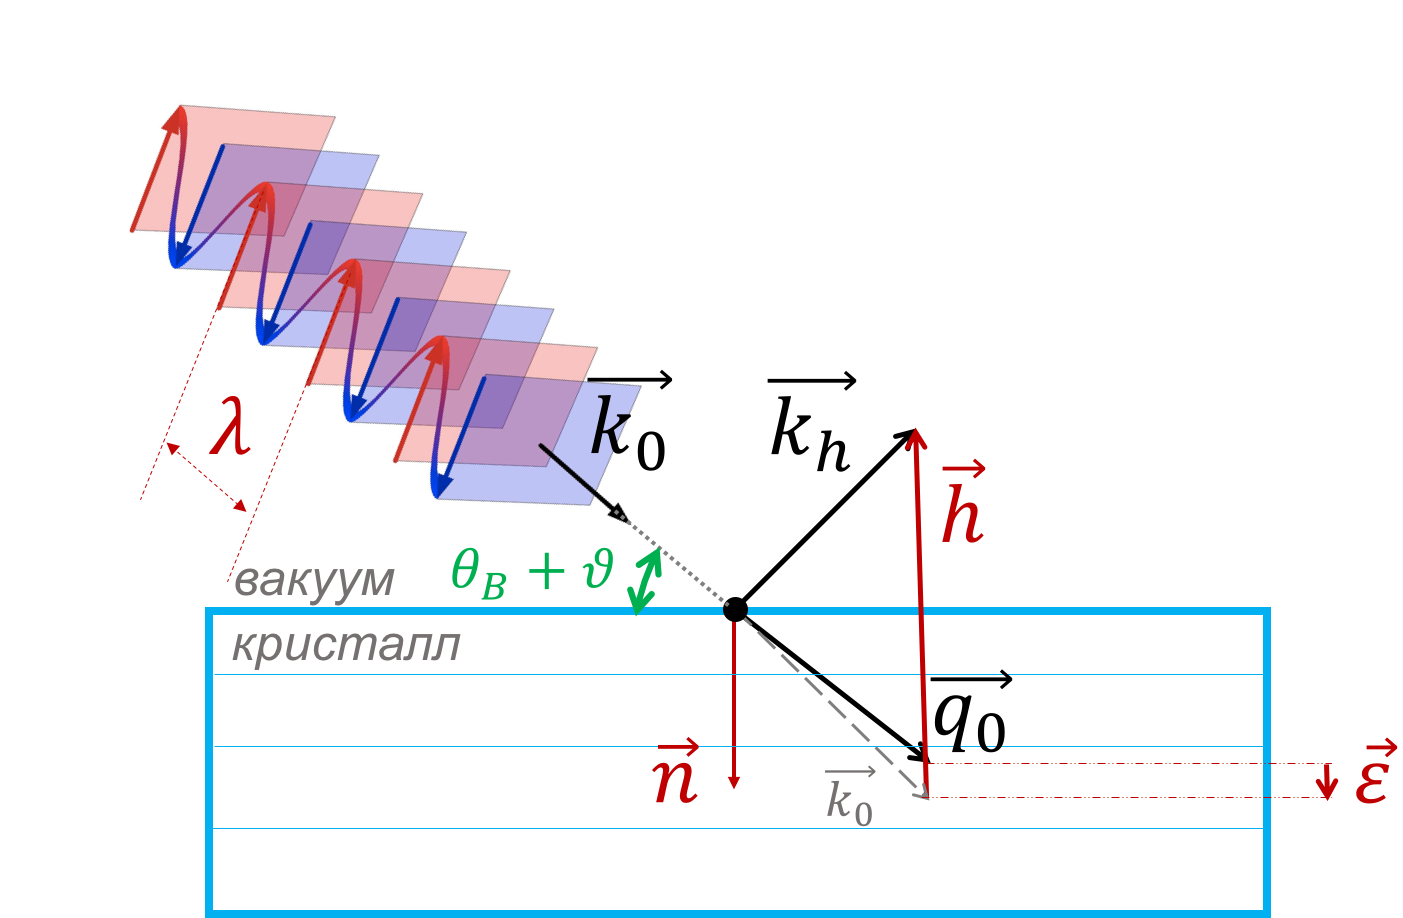
\includegraphics[width=0.6\textwidth]{images/plane_wave_vacuum.png}
    \caption{Схематичное изображение дифракции рентгеновского излучения в кристалле,
      $\vec {k}$ - волновой вектор в вакууме; $\vec {q}$ - волновой вектор в среде;
     $0$ - коэффициент для обозначения падающей волны, $h$ -  дифрагированной; $\vec{h}$ - вектор
     обратной решетки ($|h|=2\pi/d$); $\vec{n}$ - вектор нормали к поверхности, направленный внутрь объема;
     $\lambda$ - длина волны; $\vec{\varepsilon}$ - вектор аккомодации, характеризующий изменение
     волнового вектора в среде из-за преломления; $\theta_B+\vartheta$ - угол падения излучения на кристалл, для данного
     случая угол совпадает с углом Брэгга $\vartheta = 0$, т.к.  $\vec {k}_0 + \vec{h} = \vec {k}_h $}
    \label{ris:plane_wave_vacuum}
  \end{figure}

Рентгеновские лучи, как и видимый свет, распространяются параллельно и преломляются при
прохождении через границу раздела двух сред с разной оптической плотностью.
 Преломление рентгеновских лучей намного слабее, чем у видимого света, причем
 абсолютный показатель преломления рентгеновских лучей практически во всех средах
одинаков и настолько близок к единице, что их преломление не удавалось обнаружить
 в течение тридцати лет после открытия рентгеновских лучей \cite{fetisov2007}.
 Более того, для рентгеновских лучей вакуум оказывается оптически наиболее плотной средой, и луч
 при переходе в конденсированную среду увеличивает угол с нормалью к поверхности раздела сред ($n_{refr} \approx 1-10^{-5}$).
 Таким образом, волновой вектор, распространяющегося излучения отличается от своего продолжения в
 среде, но тангенциальная составляющая при переходе из одной среды в другу в соответствии с теорией о
 циркуляции сохраняется \cite{landau_8_1992}:

 \begin{equation}
   \vec{q}_0 = \vec{k}_0 + \varepsilon k_0 \cdot \vec{n}.
  \end{equation}

Тогда квадрат волнового вектора в среде:
\begin{equation}
   q_0^2 = k_0^2 + 2k_0^2 \varepsilon \cdot \gamma_0 + \cancelto{0}{k_0^4  \varepsilon^2},
   \label{eq:k_0_squred}
 \end{equation}
\noindent
где, $\gamma_0 = \cos(\vec{k}_0 \textasciicircum \vec{n})$ - косинус угла между вектором $\vec{k}_0$ и нормалью к поверхности кристалла,
последним слагаемым можно пренебречь в силу его малости ($\sim 10^{-6}$).

  Волновой вектор дифрагированной волны, в соответствии с условием Вульфа-Брэгга записывается следующим образом:
  $$\vec{k}_h = \vec{k}_0+\vec{h},$$

  \begin{equation}
     k_h^2 = \vec{k}_0^2+2k_0^2 \varepsilon \cdot \gamma_h,
     \label{eq:k_h_squred}
   \end{equation}
\noindent

где $\gamma_h = \cos(\vec{k}_0+ \vec{h} \textasciicircum \vec{n})$ - косинус угла между вектором $\vec{k}_h$ и нормалью к поверхности кристалла.

Для дальнейшего рассмотрения уравнения, связывающего амплитуду падающей и дифрагированной волн в рамках
динамической теории рассеяния, вводится параметр $\alpha$,
характеризующий степень отклонения от условия Вульфа-Брэгга \cite{Bushuev_Oreshko_2002}:
\begin{equation}
   \alpha = \frac{k_0^2-k_h^2}{k_0^2},
   \label{eq:alpha}
\end{equation}
$$  \alpha = 1 - \frac{|\vec{k}_0|^2+2|\vec{k}_0||\vec{h}|\cos(\vec{k}_0 \textasciicircum \vec{h})+|\vec{h}|^2}{k_0^2}.$$

Учитывая, что $ |h| = 2|k_0| \sin(\theta_B) $, а $\vec{k}_0 \textasciicircum \vec{h} = 90-\theta_B+\vartheta$, получим:

\begin{equation}
   \alpha = -4\sin(\theta_B)(\sin(\theta_B+\vartheta)-\sin(\theta_B)).
   \label{eq:alpha_otstroika}
\end{equation}
\noindent
Параметр $\alpha$, характеризующий отстройку падающего излучения от точного брэгговского угла удобнее ввести на
текущем этапе. Выражение (\ref{eq:alpha_otstroika}) существенно упростит
 дальнейшее рассмотрение в рамках динамической теории рассеяния.
